\scanpage{7}
\figure{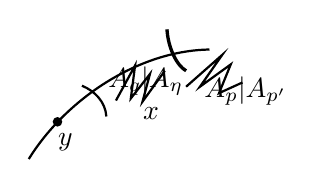
\begin{tikzpicture}[x=1.35cm,y=1.35cm]
  \draw[line width=.8pt] (0,0) .. controls (.34,.55) and (1.02,1.02) .. (1.70,1.03);
  \fill (.27,.35) circle (.045);
  \node[below right,inner sep=0pt] at (.27,.24) {$y$};
  \draw[thick] (.50,.69) .. controls (.62,.64) and (.72,.54) .. (.73,.40);
  \draw[very thick] (1.30,1.22) .. controls (1.31,1.05) and (1.39,.88) .. (1.48,.83);
  \node[inner sep=0pt] at (1.15,.43) {$x$};
  \node[inner sep=0pt] at (1.10,.73) {$\deleted{\unsure{A_q|A_{\eta}}}$};
  \node[inner sep=0pt] at (2.04,.64) {$\deleted{\unsure{A_p|A_{p'}}}$};
  \draw[thick] (.82,.55)--(1.00,.88)--(.96,.57)--(1.14,.80)--(1.07,.54)--(1.28,.83)
    (1.48,.68)--(1.82,.98)--(1.61,.68)--(1.90,.89)--(1.79,.62)--(2.01,.72);
\end{tikzpicture}}

On est amené à prouver le résultat plus fort (remplaçant $A$ par l'anneau $A_f$ d'un voisinage de $y$, pour lequel la condition d'injectivité \unsure{sera|reste|soit} donc \unsure{satisfaite|satisfait}): si $f,g:\operatorname{Spec}(A)\longrightarrow Y$ sont deux morphismes, dont les composés avec $\operatorname{Spec}(A_p)\unsure{-|\to}\operatorname{Spec}(A)$ sont identiques, ils sont identiques.

\uline{Corollaire 3} Supposons que $X$ soit loc. noeth, $Y$ \unsure{loc.} de type fini sur $S$, $S$ loc noeth (ce dernier pt est-il nécessaire ?). La donnée d'un $S$-morphisme équivaut alors à la donnée d'un $S$-hom de $\unsure{\rho|P|p}(\unsure{x|X})$ dans $\rho(Y)$

\uline{\unsure{Remarques|Remarque}} Dans la proposition plus haut\inserted{(et \unsure{$\overline{\mathrm m}$|même} le cor. 1 \unsure{modifié|modulé|seulement})}, la condition imposée à $\unsure{S|F}$ n'est pas \unsure{surabondante}.

Ex. $X=\operatorname{Spec}k[T]$ ($k$ alg. clos], \deleted{\unsure{pour}} \deleted{\unsure{toute|t.}} \deleted{partie} \inserted{\unsure{un|une|ens}} \unsure{finie|fini} $\Phi$ \deleted{de $X-\unsure{a|g|\eta}$ ($a=$ pt gén.).} \inserted{de pts fermés de $X$} on considère \deleted{$F_\Phi=\unsure{0|\coprod}\coprod_{x\in\Phi}\unsure{\varepsilon|\mathcal E|E}_x$, \unsure{soit} $F=\lim F_\Phi$}

$F=\coprod_{x\in X}\varepsilon_x$. On a donc $F_a=e$ ($a$ pt générique) Soit $\xi_x\in\Gamma(\varepsilon_x)$ l'\unsure{élmt|élmt.} \deleted{unité} \inserted{``unité''} de $\Gamma(\varepsilon_x)$, et $\xi_a=e$. Les $\xi_x$ ($x\in X$) forment un syst. cohérent qui \unsure{n'est|n'en} \unsure{pas} une section.
% archive sheet number: 6
